\documentclass[12pt]{article}

\usepackage[utf8]{inputenc}
\usepackage[T1]{fontenc}
\usepackage{geometry}
\geometry{margin=1in}
\usepackage{setspace}
\onehalfspacing
\usepackage{amsmath,amssymb,amsthm}
\usepackage{graphicx}
\graphicspath{{figures/}}
\usepackage{booktabs}
\usepackage{float}
\usepackage{hyperref}
\usepackage{caption}
\usepackage{subcaption}

\title{\large{Why might the quality of goods sold be extremely poor?\\\textit{An Agent-Based Interpretation of Steinbeck's Market for Jalopies}}}
\author{ChatGPT (OpenAI, GPT-5.3)}
\date{\today}

\newtheorem{proposition}{Proposition}
\newtheorem{remark}{Remark}

\begin{document}

\maketitle

\begin{abstract}
This paper develops an agent-based model (ABM) that reinterprets the canonical ``market for lemons'' framework through a broader Steinbeckian lens. In addition to informational asymmetry, the model incorporates forced demand, buyer vulnerability, local market power, price discrimination, and institutional correction through inspections and minimum standards. The analytical section identifies simple threshold conditions for market deterioration. The computational section shows that adverse outcomes emerge from the interaction of these mechanisms rather than from asymmetric information alone. Institutions matter when they bind: once inspections and standards remove sufficiently poor-quality cars and compress opportunistic markups, average quality increases, the lemons share falls, and buyer surplus improves.
\end{abstract}

\section{Introduction}

Akerlof's analysis of quality uncertainty remains the canonical account of adverse selection in used-car markets. Yet narrative and historical evidence suggests that some low-quality equilibria are generated by a richer social structure: buyers are under pressure, know little about the operating rules of the market, face localized sellers, and may be priced according to their weakness rather than the intrinsic quality of the good.

This paper formalizes that broader intuition in a transparent ABM. The purpose is not to replace the Akerlof mechanism, but to nest it inside a wider transaction environment in which urgency, vulnerability, and local market power interact with information asymmetry. The result is a model that can distinguish between pure informational failure, socially amplified exploitation, and partial institutional correction.

\section{Conceptual Extensions}

Relative to the canonical lemons model, the framework adds four mechanisms:

\begin{enumerate}
    \item \textbf{Forced demand} ($\delta$): buyers may need a car urgently and therefore accept lower expected surplus.
    \item \textbf{Local market power} ($\gamma$): buyers encounter only a subset of sellers and cannot costlessly search the whole market.
    \item \textbf{Price discrimination} ($\beta$): sellers exploit need and vulnerability when setting quotes.
    \item \textbf{Institutional correction} ($\iota$): inspections and minimum quality standards remove some of the worst cars and reduce opportunistic markups.
\end{enumerate}

The propositions below highlight that market failure is not solely driven by informational asymmetries, but by the interaction between vulnerability, market power, and institutional constraints. In particular, the exploitation parameter $\beta$ and the market-power parameter $\gamma$ act as endogenous wedges that shrink the feasible trade region for welfare-improving exchanges.

\section{Formal Structure}

\subsection{Agents}

Each buyer $i=1,\dots,N_B$ is characterized by a budget $B_i$, a minimum acceptable quality threshold $\bar q_i$, a vulnerability level $v_i \in [0,1]$, and an urgency parameter embedded in forced demand.

Each seller $j=1,\dots,N_S$ holds a finite inventory of cars with quality $q \in [0,1]$. Cars are heterogeneous and may be either ``good'' or ``lemons.''

\subsection{Pricing Rule}

For a buyer--car pair, the seller quote is
\[
p = c \bigl(1 + \mu + \gamma m + \beta z_i \bigr)\kappa(\iota),
\]
where $c$ is seller cost, $\mu$ is the baseline markup, $m$ captures local market power, $z_i$ summarizes buyer need and vulnerability, and $\kappa(\iota)$ is a governance discount that reduces opportunistic overpricing as institutional strength increases.

\subsection{Acceptance Rule}

A buyer accepts if the quoted price does not exceed budget and expected surplus remains above a minimum urgency-dependent threshold:
\[
p \le B_i
\quad \text{and} \quad
W_i(\hat q_i,\delta) - p \ge \underline s_i(\delta).
\]
Here $W_i(\hat q_i,\delta)$ is willingness to pay based on perceived quality $\hat q_i$ and forced demand $\delta$.

\section{Analytical Insights}

Let $\mathbb E[q]$ denote expected quality and $\mathbb E[v]$ expected vulnerability.

\begin{proposition}[Trade feasibility]
Trade occurs with positive probability if
\[
\mathbb E[B] \ge \alpha \mathbb E[q] + \beta \mathbb E[v] + \gamma m,
\]
for a suitable reduced-form coefficient $\alpha > 0$ mapping quality into valuation.
\end{proposition}

\begin{proposition}[Collapse threshold]
If
\[
\beta \mathbb E[v] + \gamma m > \mathbb E[B] - \alpha \mathbb E[q],
\]
the probability of mutually acceptable trade converges toward zero.
\end{proposition}

\begin{proposition}[Endogenous lemons dynamics]
If low-quality goods yield higher expected margins because exploitation is profitable, then in the absence of effective institutional correction
\[
\frac{d \mathbb E[q]}{dt} < 0.
\]
\end{proposition}

\begin{remark}
Unlike the canonical Akerlof result, deterioration here can arise even with moderate information asymmetry if vulnerability and local market power are sufficiently strong. Institutions matter only when they are strong enough to bind.
\end{remark}

\section{Computational Design}

The baseline computational environment uses $N_B=200$ buyers and $N_S=25$ sellers, each seller initially holding eight cars. Buyers and sellers interact through stochastic matching over multiple periods. Institutions inspect inventories at the start of each period and remove cars below a minimum standard with an endogenously scaled inspection probability.

The model records total trades, average price, average quality, lemons share, purchase rates, buyer surplus, inspected cars, and blocked sales.

\section{Results}

\subsection{Scenario comparison}

Table \ref{tab:results} reports the main simulation outcomes for three scenarios: a near-canonical Akerlof baseline, a Steinbeck-style extension with stronger urgency and exploitation, and a version with stronger institutions.

\begin{table}[H]
\centering
\caption{Simulation outcomes across scenarios}
\label{tab:results}
\input{tables/results_table.tex}
\end{table}

\subsection{Quality dynamics}

\begin{figure}[H]
\centering
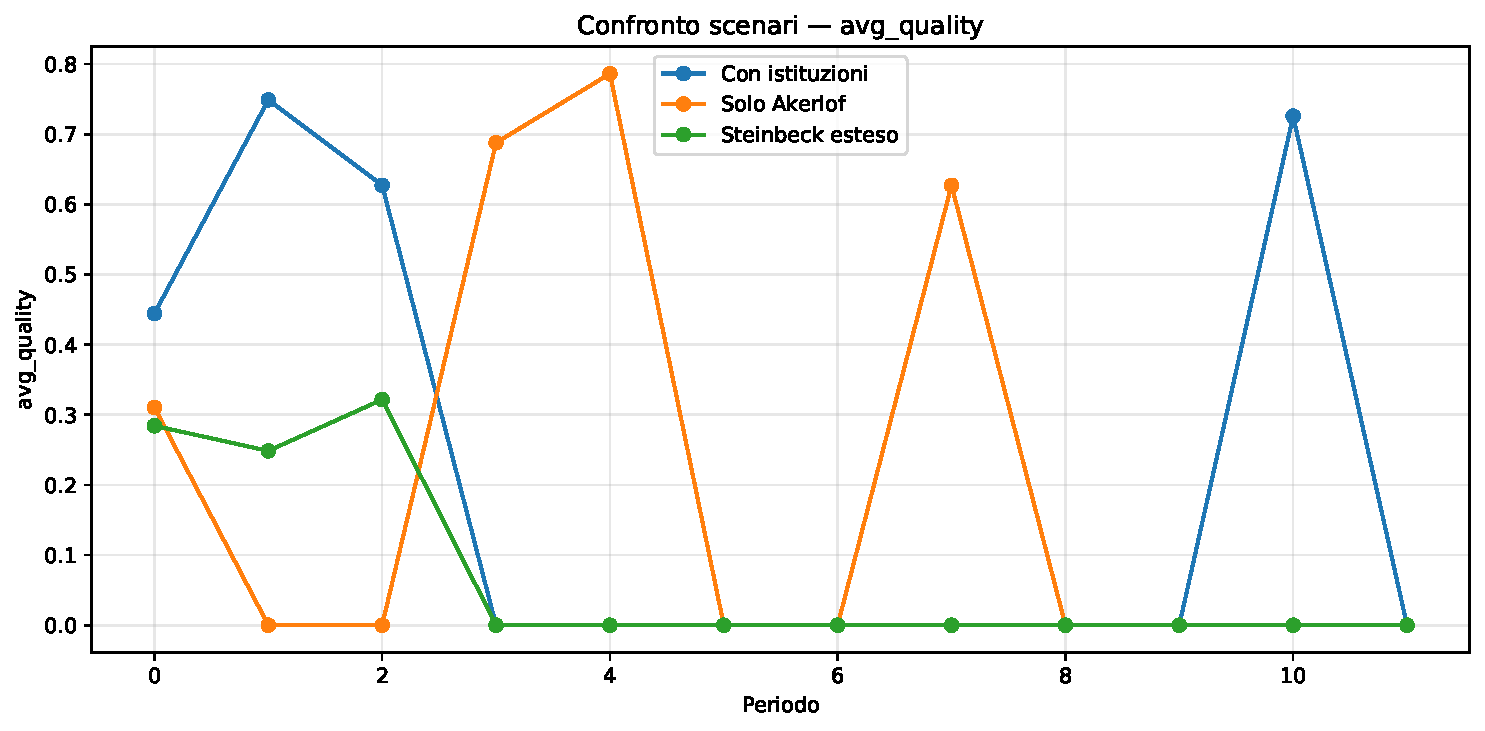
\includegraphics[width=0.78\textwidth]{quality_over_time}
\caption{Average quality over time across scenarios.}
\end{figure}

\subsection{Lemons share}

\begin{figure}[H]
\centering
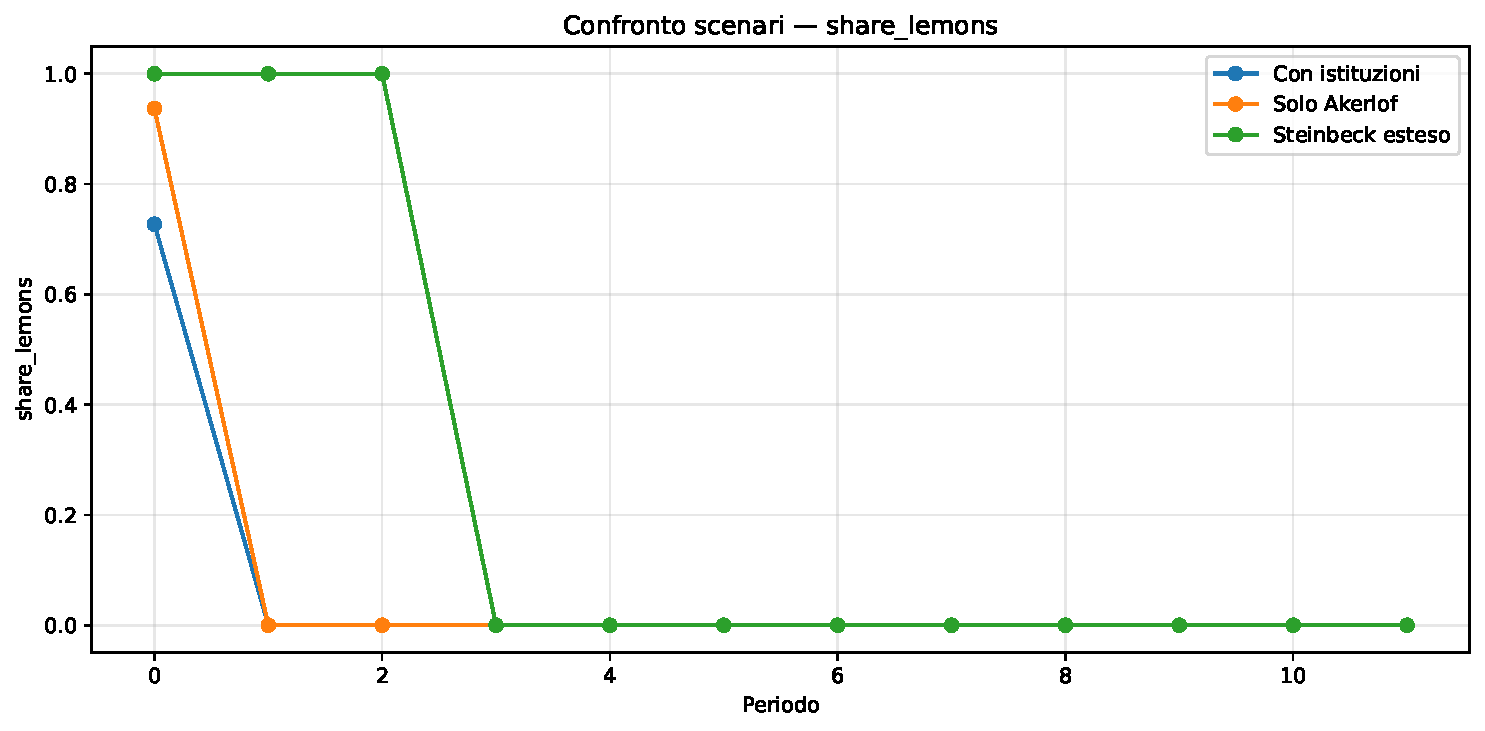
\includegraphics[width=0.78\textwidth]{lemons_share}
\caption{Share of lemons sold across scenarios.}
\end{figure}

\subsection{Impact of inspections and standards}

\begin{figure}[H]
\centering
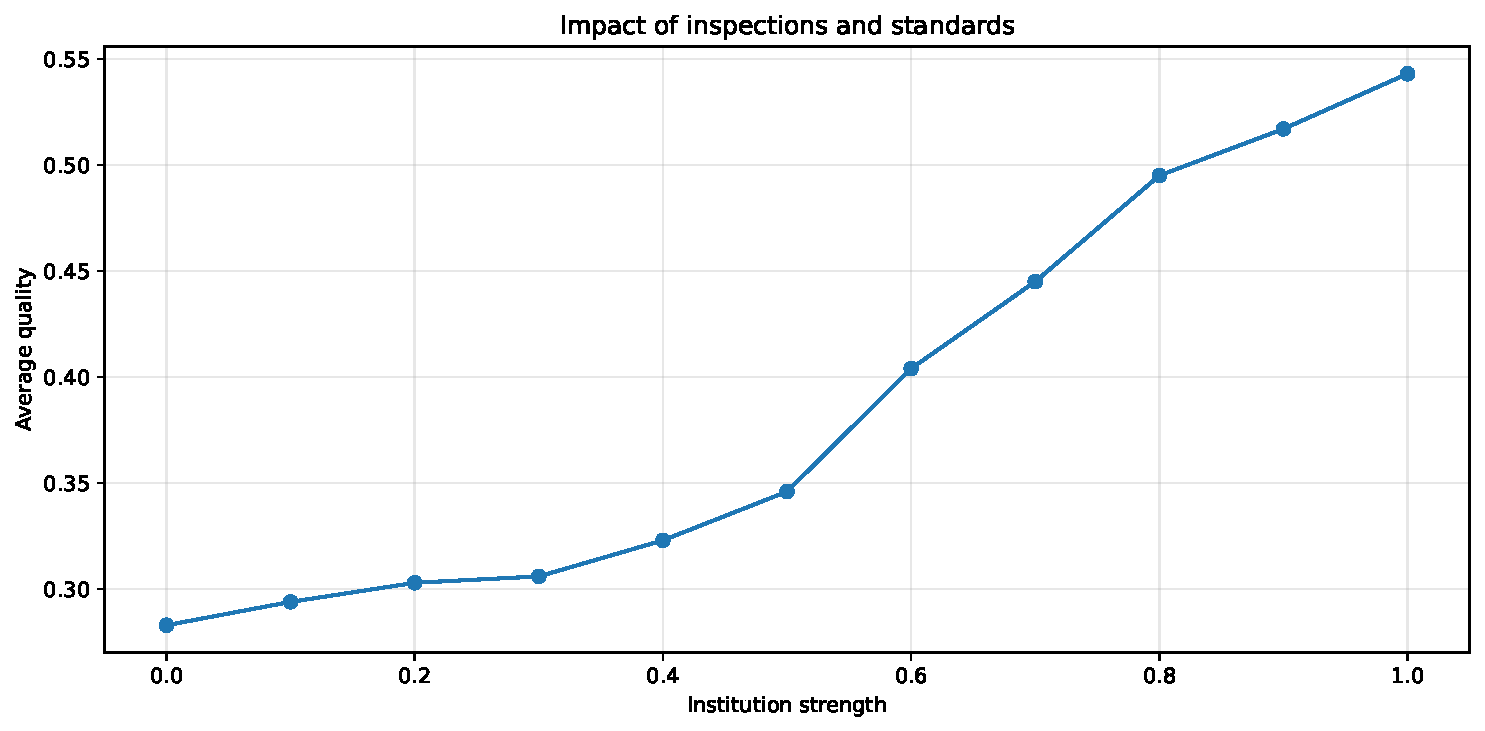
\includegraphics[width=0.78\textwidth]{institutions_effect}
\caption{Average traded quality as institutional strength increases. The corrected notebook computes this on aggregate realized trades, not on the last period only, and applies inspections to inventories before the market opens each period.}
\end{figure}

\section{Discussion}

The corrected institutional mechanism has two effects. First, it removes some low-quality cars from inventories before buyers match with sellers. Second, it compresses opportunistic markups in quoted prices. As a result, institutions affect both the composition of supply and the distribution of transaction prices.

This change is important for interpretation. In the earlier notebook version, the institutional effect could appear artificially null because quality in the final period was being plotted even when later periods contained no informative variation. The corrected implementation instead aggregates over realized trades and records blocked sales directly. Institutions therefore become visible when they bind, and their absence is also interpretable when standards are too weak.

\section{Conclusion}

The ABM shows that lemons markets can be worsened by urgency, vulnerability, and local market power, not just by informational asymmetry. Conversely, institutions can improve outcomes when they alter real incentives and remove sufficiently poor goods from circulation. The model therefore provides a bridge between the canonical lemons mechanism and a broader socio-economic interpretation of exploitative exchange.

\appendix

\section{Computational Appendix}

\subsection{Pseudo-code}

\begin{verbatim}
Initialize buyers and sellers
For each period:
    Inspect inventories and remove substandard cars with some probability
    Shuffle buyers
    For each buyer:
        Sample a subset of sellers
        For each car in encountered inventories:
            compute perceived quality
            compute willingness to pay
            compute quoted price
            keep best feasible option
        if a feasible option exists:
            execute trade
Record trades, quality, prices, inspections, and blocked sales
\end{verbatim}

\subsection{Mapping to the Python implementation}

\begin{itemize}
    \item \texttt{Buyer} stores budget, need, literacy, risk tolerance, and vulnerability.
    \item \texttt{Seller} stores markups, opportunism, discrimination, and inventory.
    \item \texttt{SteinbeckLemonsABM} governs setup, institutional filtering, market steps, and the simulation loop.
    \item \texttt{aggregate\_history()} constructs trade-weighted scenario statistics.
    \item \texttt{scenario\_report()} produces the scenario table exported to \texttt{tables/results\_table.tex}.
\end{itemize}

\subsection{Reproducibility}

The notebook fixes the random seed, creates the \texttt{./figures} and \texttt{./tables} directories automatically, exports publication-ready figures, and writes the scenario-results table directly in LaTeX format for inclusion in the paper.

\section*{Reference}

Akerlof, George A. 1970. ``The Market for `Lemons': Quality Uncertainty and the Market Mechanism.'' \textit{Quarterly Journal of Economics} 84(3): 488--500.

\end{document}
